\subsection{Quadrilateral AFEM and neural-transfer comparison}

We discretize (1) with continuous $Q_1\times Q_1$ finite elements on
hierarchically refined quadrilateral meshes and use backward Euler with
$\tau=0.01$.  The recovery estimator is
$\eta_K=\lVert G(\nabla\phi_h)-\nabla\phi_h\rVert_{L^2(K)}$.  In the
classical run, deal.II's \texttt{SolutionTransfer} transfers the finite element
solution after refinement and coarsening.  In the neural run, a
$2$--$40$--$40$--$40$--$1$ tanh network interpolates the previous
$\phi_h$ on the new mesh; the mixed finite element solve then recomputes both
$\phi_h$ and $\mu_h$.  Both methods use the same marking fractions,
$\theta_r=0.6$ and $\theta_c=0.4$, and five initial adaptation cycles.

Tables~\ref{tab:ex1-transfer} and~\ref{tab:ex2-transfer} report the computed
$L^2$ errors at $t=0.05$.  The DoF count includes both scalar components.

\begin{table}[htbp]
  \centering
  \caption{Example 1 on quadrilateral meshes at $t=0.05$.}
  \label{tab:ex1-transfer}
  \begin{tabular}{lrrr}
    \hline
    Transfer method & DoFs & $\lVert\phi-\phi_h\rVert_{L^2}$ &
      $\lVert\mu-\mu_h\rVert_{L^2}$ \\
    \hline
    Classical AFEM & 19,158 & $1.2891\times10^{-3}$ & $3.0654\times10^{-2}$ \\
    Neural interpolation & 19,158 & $1.4174\times10^{-3}$ & $3.0239\times10^{-2}$ \\
    \hline
  \end{tabular}
\end{table}

\begin{table}[htbp]
  \centering
  \caption{Example 2 on quadrilateral meshes at $t=0.05$ (preliminary).}
  \label{tab:ex2-transfer}
  \begin{tabular}{lrrr}
    \hline
    Transfer method & DoFs & $\lVert\phi-\phi_h\rVert_{L^2}$ &
      $\lVert\mu-\mu_h\rVert_{L^2}$ \\
    \hline
    Classical AFEM & 2,462 & $1.1588\times10^{-1}$ & $1.1421$ \\
    Neural interpolation & 2,486 & $1.1284\times10^{-1}$ & $1.0962$ \\
    \hline
  \end{tabular}
\end{table}

\begin{figure}[htbp]
  \centering
  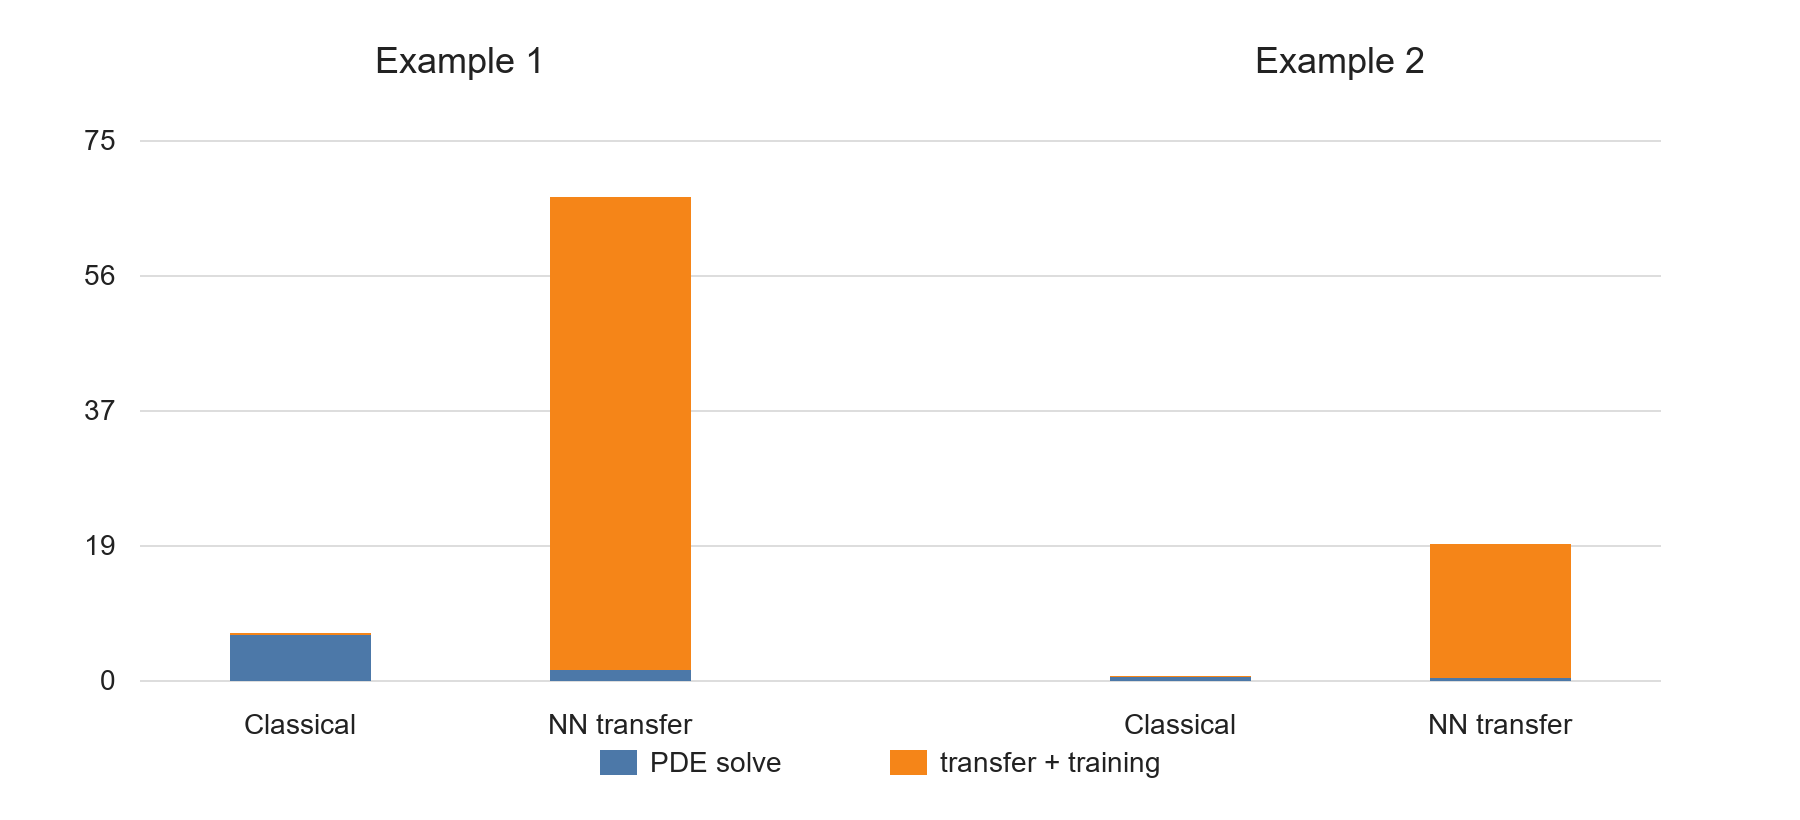
\includegraphics[width=0.88\textwidth]{cost-comparison.png}
  \caption{Measured wall time through $t=0.05$.  Neural training dominates
  the present CPU implementation: 65.25 s in Example 1 and 18.43 s in
  Example 2, compared with classical transfer costs below 0.13 s.}
  \label{fig:transfer-cost}
\end{figure}

The neural transfer preserves the final accuracy in Example 1: relative to
classical transfer, the error in $\phi$ is 9.95\% larger and the error in
$\mu$ is 1.35\% smaller.  The current implementation does not yet provide a
cost advantage because repeated CPU L-BFGS training is substantially more
expensive than finite element interpolation.

Example 2 exposes a fail-fast limitation.  With the prescribed fixed-fraction
marking, five initial cycles leave only 290 mixed DoFs around the Gaussian.
The recovery indicator therefore begins from an under-resolved peak, and the
absolute $\phi$ error remains approximately $1.1\times10^{-1}$ at $t=0.05$.
The classical and neural results agree closely, so the transfer comparison is
internally consistent, but these values should not yet be presented as a
high-accuracy Gaussian benchmark.  The next test should impose a minimum local
resolution near the initial peak (or add initial global refinements) before
comparing transfer methods.

The current manuscript formula for Example 2 uses
$0.3\cos(2\pi t)$ for both center coordinates.  Consequently, the implemented
peak oscillates along the diagonal rather than following a circular path.  If
circular motion is intended, the second center coordinate should be changed to
$0.3\sin(2\pi t)$ in both the manuscript and code.
